\documentclass[]{article}
\usepackage{lmodern}
\usepackage{amssymb,amsmath}
\usepackage{ifxetex,ifluatex}
\usepackage{fixltx2e} % provides \textsubscript
\ifnum 0\ifxetex 1\fi\ifluatex 1\fi=0 % if pdftex
  \usepackage[T1]{fontenc}
  \usepackage[utf8]{inputenc}
\else % if luatex or xelatex
  \ifxetex
    \usepackage{mathspec}
  \else
    \usepackage{fontspec}
  \fi
  \defaultfontfeatures{Ligatures=TeX,Scale=MatchLowercase}
\fi
% use upquote if available, for straight quotes in verbatim environments
\IfFileExists{upquote.sty}{\usepackage{upquote}}{}
% use microtype if available
\IfFileExists{microtype.sty}{%
\usepackage{microtype}
\UseMicrotypeSet[protrusion]{basicmath} % disable protrusion for tt fonts
}{}
\usepackage[margin=1in]{geometry}
\usepackage{hyperref}
\hypersetup{unicode=true,
            pdftitle={Creating-a-master},
            pdfborder={0 0 0},
            breaklinks=true}
\urlstyle{same}  % don't use monospace font for urls
\usepackage{color}
\usepackage{fancyvrb}
\newcommand{\VerbBar}{|}
\newcommand{\VERB}{\Verb[commandchars=\\\{\}]}
\DefineVerbatimEnvironment{Highlighting}{Verbatim}{commandchars=\\\{\}}
% Add ',fontsize=\small' for more characters per line
\usepackage{framed}
\definecolor{shadecolor}{RGB}{248,248,248}
\newenvironment{Shaded}{\begin{snugshade}}{\end{snugshade}}
\newcommand{\KeywordTok}[1]{\textcolor[rgb]{0.13,0.29,0.53}{\textbf{#1}}}
\newcommand{\DataTypeTok}[1]{\textcolor[rgb]{0.13,0.29,0.53}{#1}}
\newcommand{\DecValTok}[1]{\textcolor[rgb]{0.00,0.00,0.81}{#1}}
\newcommand{\BaseNTok}[1]{\textcolor[rgb]{0.00,0.00,0.81}{#1}}
\newcommand{\FloatTok}[1]{\textcolor[rgb]{0.00,0.00,0.81}{#1}}
\newcommand{\ConstantTok}[1]{\textcolor[rgb]{0.00,0.00,0.00}{#1}}
\newcommand{\CharTok}[1]{\textcolor[rgb]{0.31,0.60,0.02}{#1}}
\newcommand{\SpecialCharTok}[1]{\textcolor[rgb]{0.00,0.00,0.00}{#1}}
\newcommand{\StringTok}[1]{\textcolor[rgb]{0.31,0.60,0.02}{#1}}
\newcommand{\VerbatimStringTok}[1]{\textcolor[rgb]{0.31,0.60,0.02}{#1}}
\newcommand{\SpecialStringTok}[1]{\textcolor[rgb]{0.31,0.60,0.02}{#1}}
\newcommand{\ImportTok}[1]{#1}
\newcommand{\CommentTok}[1]{\textcolor[rgb]{0.56,0.35,0.01}{\textit{#1}}}
\newcommand{\DocumentationTok}[1]{\textcolor[rgb]{0.56,0.35,0.01}{\textbf{\textit{#1}}}}
\newcommand{\AnnotationTok}[1]{\textcolor[rgb]{0.56,0.35,0.01}{\textbf{\textit{#1}}}}
\newcommand{\CommentVarTok}[1]{\textcolor[rgb]{0.56,0.35,0.01}{\textbf{\textit{#1}}}}
\newcommand{\OtherTok}[1]{\textcolor[rgb]{0.56,0.35,0.01}{#1}}
\newcommand{\FunctionTok}[1]{\textcolor[rgb]{0.00,0.00,0.00}{#1}}
\newcommand{\VariableTok}[1]{\textcolor[rgb]{0.00,0.00,0.00}{#1}}
\newcommand{\ControlFlowTok}[1]{\textcolor[rgb]{0.13,0.29,0.53}{\textbf{#1}}}
\newcommand{\OperatorTok}[1]{\textcolor[rgb]{0.81,0.36,0.00}{\textbf{#1}}}
\newcommand{\BuiltInTok}[1]{#1}
\newcommand{\ExtensionTok}[1]{#1}
\newcommand{\PreprocessorTok}[1]{\textcolor[rgb]{0.56,0.35,0.01}{\textit{#1}}}
\newcommand{\AttributeTok}[1]{\textcolor[rgb]{0.77,0.63,0.00}{#1}}
\newcommand{\RegionMarkerTok}[1]{#1}
\newcommand{\InformationTok}[1]{\textcolor[rgb]{0.56,0.35,0.01}{\textbf{\textit{#1}}}}
\newcommand{\WarningTok}[1]{\textcolor[rgb]{0.56,0.35,0.01}{\textbf{\textit{#1}}}}
\newcommand{\AlertTok}[1]{\textcolor[rgb]{0.94,0.16,0.16}{#1}}
\newcommand{\ErrorTok}[1]{\textcolor[rgb]{0.64,0.00,0.00}{\textbf{#1}}}
\newcommand{\NormalTok}[1]{#1}
\usepackage{graphicx,grffile}
\makeatletter
\def\maxwidth{\ifdim\Gin@nat@width>\linewidth\linewidth\else\Gin@nat@width\fi}
\def\maxheight{\ifdim\Gin@nat@height>\textheight\textheight\else\Gin@nat@height\fi}
\makeatother
% Scale images if necessary, so that they will not overflow the page
% margins by default, and it is still possible to overwrite the defaults
% using explicit options in \includegraphics[width, height, ...]{}
\setkeys{Gin}{width=\maxwidth,height=\maxheight,keepaspectratio}
\IfFileExists{parskip.sty}{%
\usepackage{parskip}
}{% else
\setlength{\parindent}{0pt}
\setlength{\parskip}{6pt plus 2pt minus 1pt}
}
\setlength{\emergencystretch}{3em}  % prevent overfull lines
\providecommand{\tightlist}{%
  \setlength{\itemsep}{0pt}\setlength{\parskip}{0pt}}
\setcounter{secnumdepth}{0}
% Redefines (sub)paragraphs to behave more like sections
\ifx\paragraph\undefined\else
\let\oldparagraph\paragraph
\renewcommand{\paragraph}[1]{\oldparagraph{#1}\mbox{}}
\fi
\ifx\subparagraph\undefined\else
\let\oldsubparagraph\subparagraph
\renewcommand{\subparagraph}[1]{\oldsubparagraph{#1}\mbox{}}
\fi

%%% Use protect on footnotes to avoid problems with footnotes in titles
\let\rmarkdownfootnote\footnote%
\def\footnote{\protect\rmarkdownfootnote}

%%% Change title format to be more compact
\usepackage{titling}

% Create subtitle command for use in maketitle
\newcommand{\subtitle}[1]{
  \posttitle{
    \begin{center}\large#1\end{center}
    }
}

\setlength{\droptitle}{-2em}
  \title{Creating-a-master}
  \pretitle{\vspace{\droptitle}\centering\huge}
  \posttitle{\par}
  \author{}
  \preauthor{}\postauthor{}
  \date{}
  \predate{}\postdate{}


\begin{document}
\maketitle

\subsection{Situation}\label{situation}

There are a lot of various files that need to be combined such that the
table can be easily queried.

Here is what the current ``Master'' looks like write below.

\begin{figure}
\centering
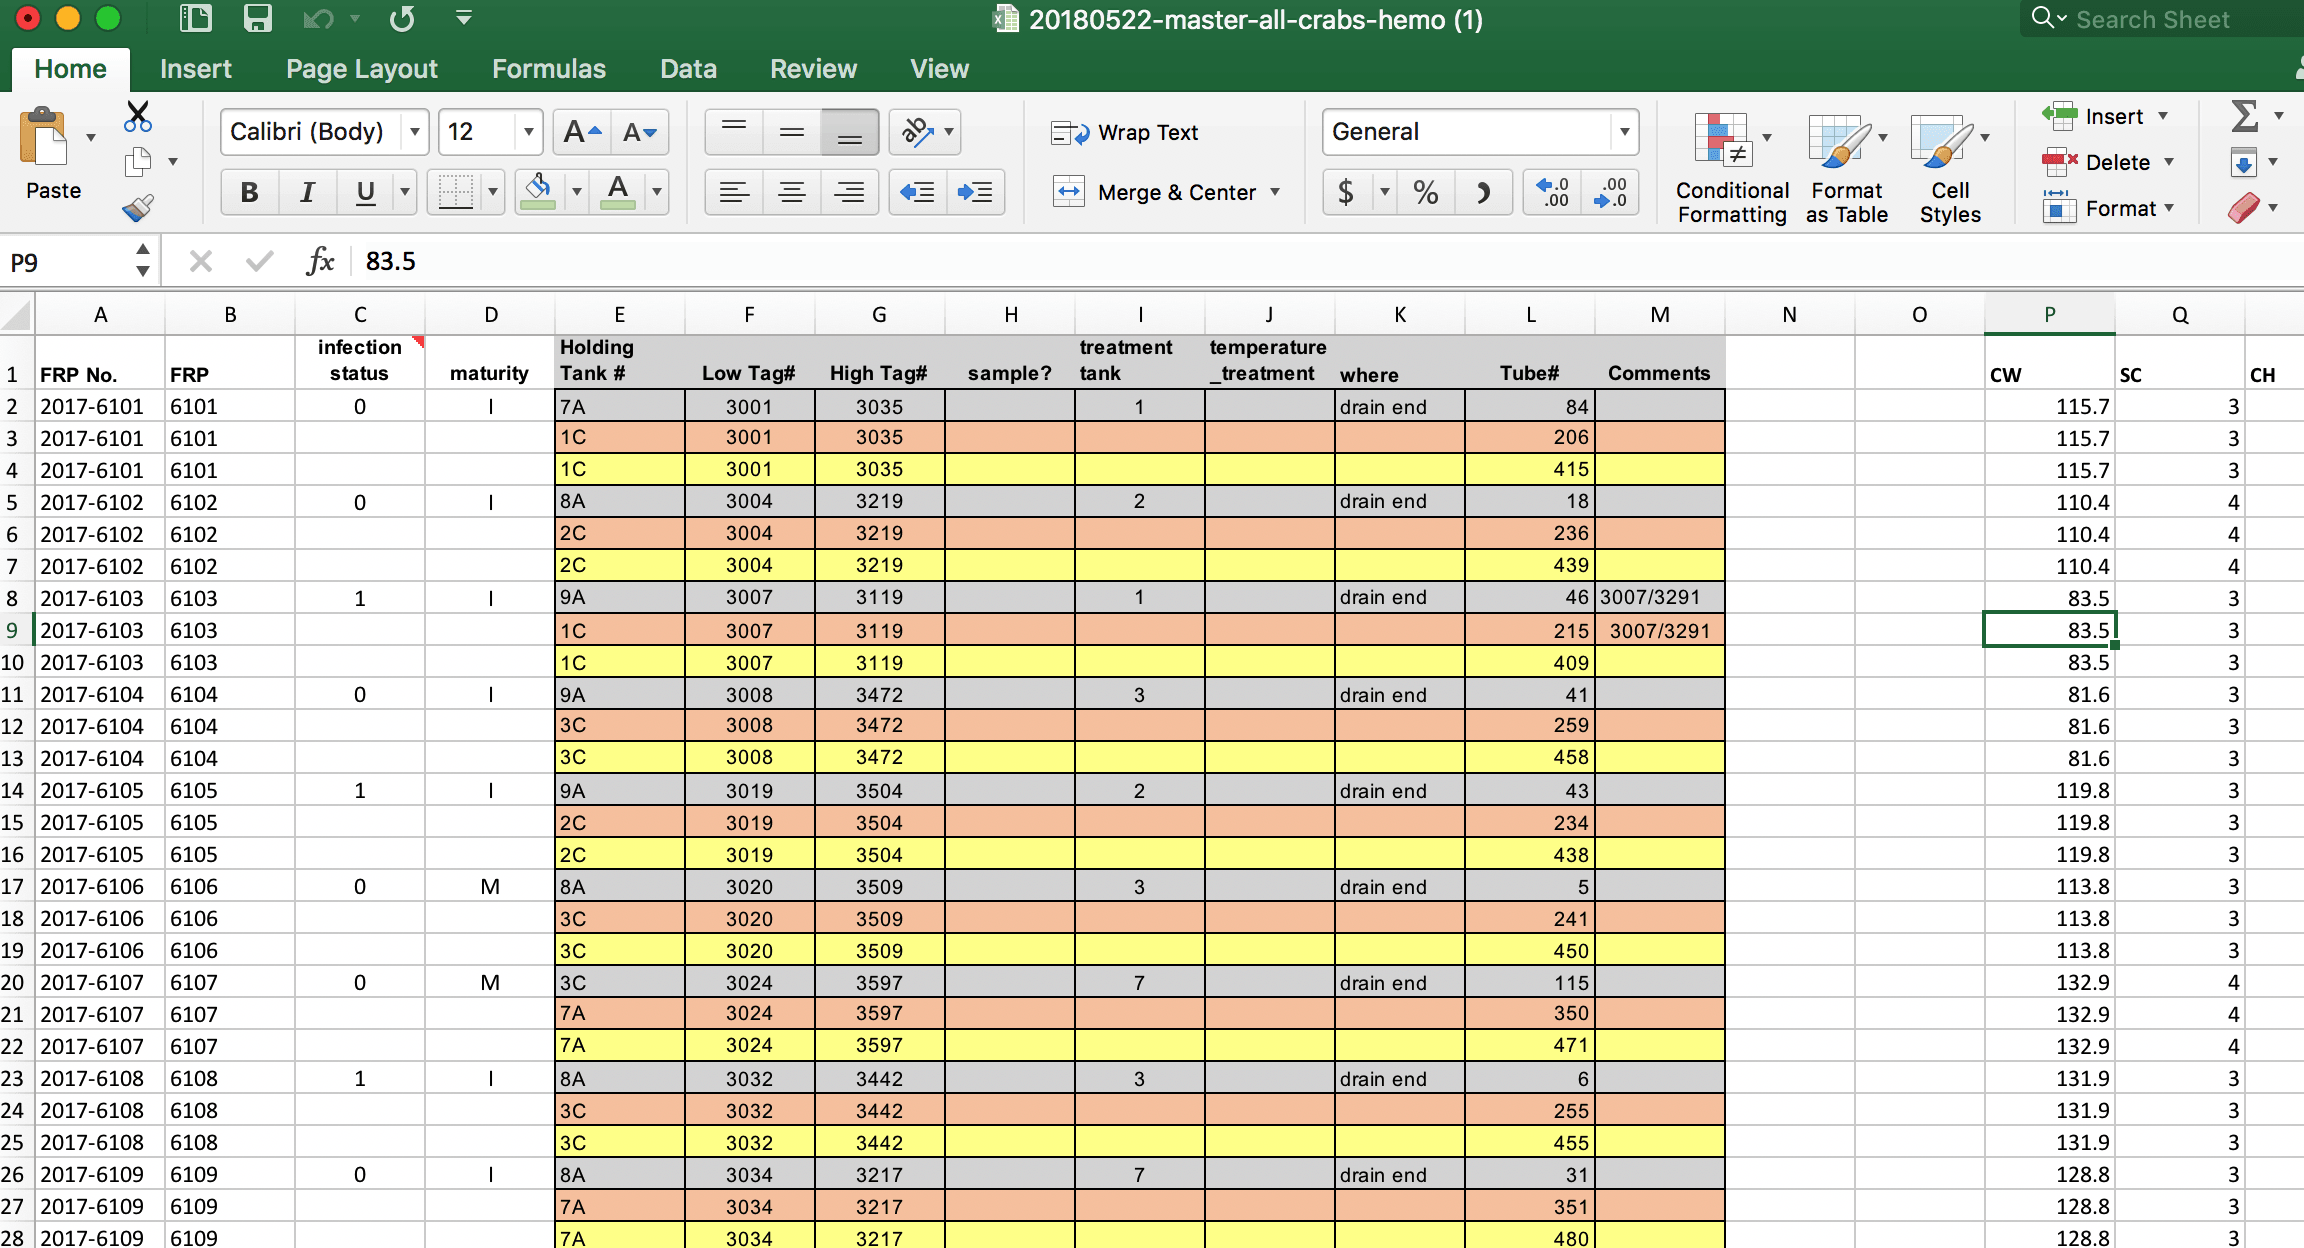
\includegraphics{img/master.png}
\caption{ss}
\end{figure}

\begin{Shaded}
\begin{Highlighting}[]
\NormalTok{    prim_master <-}\StringTok{ }\KeywordTok{read_csv}\NormalTok{(}\StringTok{"../data/20180522-master-all-crabs-hemo-mod3.csv"}\NormalTok{)}
\end{Highlighting}
\end{Shaded}

\begin{verbatim}
## Parsed with column specification:
## cols(
##   `FRP No.` = col_character(),
##   FRP = col_integer(),
##   `infection_cpcr-d0` = col_integer(),
##   maturity = col_character(),
##   CW = col_double(),
##   SC = col_integer(),
##   CH = col_double(),
##   holdtank = col_character(),
##   TREATMENT = col_character(),
##   lowtag = col_integer(),
##   hightag = col_integer(),
##   treattank = col_integer(),
##   where = col_character(),
##   tube_no = col_character()
## )
\end{verbatim}

\begin{Shaded}
\begin{Highlighting}[]
\BuiltInTok{pwd}
\end{Highlighting}
\end{Shaded}

\begin{verbatim}
## /Users/sr320/Documents/GitHub/Roberts-crab/Rmd
\end{verbatim}

\begin{Shaded}
\begin{Highlighting}[]
\KeywordTok{head}\NormalTok{(prim_master)}
\end{Highlighting}
\end{Shaded}

\begin{verbatim}
## # A tibble: 6 x 14
##   `FRP No.`   FRP `infection_cpcr-d0` maturity    CW    SC    CH holdtank
##   <chr>     <int>               <int> <chr>    <dbl> <int> <dbl> <chr>   
## 1 2017-6101  6101                   0 I         116.     3  20.4 7A      
## 2 2017-6101  6101                   0 I         116.     3  20.4 1C      
## 3 2017-6101  6101                   0 I         116.     3  20.4 1C      
## 4 2017-6102  6102                   0 I         110.     4  15.4 8A      
## 5 2017-6102  6102                   0 I         110.     4  15.4 2C      
## 6 2017-6102  6102                   0 I         110.     4  15.4 2C      
## # ... with 6 more variables: TREATMENT <chr>, lowtag <int>, hightag <int>,
## #   treattank <int>, where <chr>, tube_no <chr>
\end{verbatim}

\begin{Shaded}
\begin{Highlighting}[]
\NormalTok{prim_master}
\end{Highlighting}
\end{Shaded}

\begin{verbatim}
## # A tibble: 476 x 14
##    `FRP No.`   FRP `infection_cpcr-d0` maturity    CW    SC    CH holdtank
##    <chr>     <int>               <int> <chr>    <dbl> <int> <dbl> <chr>   
##  1 2017-6101  6101                   0 I        116.      3  20.4 7A      
##  2 2017-6101  6101                   0 I        116.      3  20.4 1C      
##  3 2017-6101  6101                   0 I        116.      3  20.4 1C      
##  4 2017-6102  6102                   0 I        110.      4  15.4 8A      
##  5 2017-6102  6102                   0 I        110.      4  15.4 2C      
##  6 2017-6102  6102                   0 I        110.      4  15.4 2C      
##  7 2017-6103  6103                   1 I         83.5     3  10.8 9A      
##  8 2017-6103  6103                   1 I         83.5     3  10.8 1C      
##  9 2017-6103  6103                   1 I         83.5     3  10.8 1C      
## 10 2017-6104  6104                   0 I         81.6     3  11   9A      
## # ... with 466 more rows, and 6 more variables: TREATMENT <chr>,
## #   lowtag <int>, hightag <int>, treattank <int>, where <chr>,
## #   tube_no <chr>
\end{verbatim}

\begin{Shaded}
\begin{Highlighting}[]
\NormalTok{df <-}\StringTok{ }\NormalTok{prim_master }\OperatorTok\StringTok{ }
\StringTok{  }\KeywordTok{group_by}\NormalTok{(FRP) }\OperatorTok\StringTok{ }
\StringTok{  }\KeywordTok{mutate}\NormalTok{(}\DataTypeTok{grouped_id =} \KeywordTok{row_number}\NormalTok{())}
\NormalTok{df}
\end{Highlighting}
\end{Shaded}

\begin{verbatim}
## # A tibble: 476 x 15
## # Groups:   FRP [182]
##    `FRP No.`   FRP `infection_cpcr-d0` maturity    CW    SC    CH holdtank
##    <chr>     <int>               <int> <chr>    <dbl> <int> <dbl> <chr>   
##  1 2017-6101  6101                   0 I        116.      3  20.4 7A      
##  2 2017-6101  6101                   0 I        116.      3  20.4 1C      
##  3 2017-6101  6101                   0 I        116.      3  20.4 1C      
##  4 2017-6102  6102                   0 I        110.      4  15.4 8A      
##  5 2017-6102  6102                   0 I        110.      4  15.4 2C      
##  6 2017-6102  6102                   0 I        110.      4  15.4 2C      
##  7 2017-6103  6103                   1 I         83.5     3  10.8 9A      
##  8 2017-6103  6103                   1 I         83.5     3  10.8 1C      
##  9 2017-6103  6103                   1 I         83.5     3  10.8 1C      
## 10 2017-6104  6104                   0 I         81.6     3  11   9A      
## # ... with 466 more rows, and 7 more variables: TREATMENT <chr>,
## #   lowtag <int>, hightag <int>, treattank <int>, where <chr>,
## #   tube_no <chr>, grouped_id <int>
\end{verbatim}

\begin{Shaded}
\begin{Highlighting}[]
\NormalTok{dfhack <-}\StringTok{ }\NormalTok{df }\OperatorTok\StringTok{ }
\StringTok{  }\KeywordTok{spread}\NormalTok{(grouped_id, tube_no)}
\end{Highlighting}
\end{Shaded}

\begin{Shaded}
\begin{Highlighting}[]
\NormalTok{dfhack}
\end{Highlighting}
\end{Shaded}

\begin{verbatim}
## # A tibble: 340 x 16
## # Groups:   FRP [182]
##    `FRP No.`   FRP `infection_cpcr-d0` maturity    CW    SC    CH holdtank
##    <chr>     <int>               <int> <chr>    <dbl> <int> <dbl> <chr>   
##  1 2017-6101  6101                   0 I        116.      3  20.4 7A      
##  2 2017-6101  6101                   0 I        116.      3  20.4 1C      
##  3 2017-6102  6102                   0 I        110.      4  15.4 8A      
##  4 2017-6102  6102                   0 I        110.      4  15.4 2C      
##  5 2017-6103  6103                   1 I         83.5     3  10.8 9A      
##  6 2017-6103  6103                   1 I         83.5     3  10.8 1C      
##  7 2017-6104  6104                   0 I         81.6     3  11   9A      
##  8 2017-6104  6104                   0 I         81.6     3  11   3C      
##  9 2017-6105  6105                   1 I        120.      3  19.2 9A      
## 10 2017-6105  6105                   1 I        120.      3  19.2 2C      
## # ... with 330 more rows, and 8 more variables: TREATMENT <chr>,
## #   lowtag <int>, hightag <int>, treattank <int>, where <chr>, `1` <chr>,
## #   `2` <chr>, `3` <chr>
\end{verbatim}

\begin{Shaded}
\begin{Highlighting}[]
\KeywordTok{write_csv}\NormalTok{(dfhack, }\StringTok{"../analyses/dfhack.csv"}\NormalTok{)}
\end{Highlighting}
\end{Shaded}

\subsection{Open in Excel. .}\label{open-in-excel.-.}

magic crap

See video

\url{http://owl.fish.washington.edu/whale/excel_crap.mov}

dfhack2 is the file once hacked up with Excel

\begin{Shaded}
\begin{Highlighting}[]
\NormalTok{dfhack2 <-}\StringTok{ }\KeywordTok{read_csv}\NormalTok{(}\StringTok{"../analyses/dfhack.csv"}\NormalTok{)}
\end{Highlighting}
\end{Shaded}

\begin{verbatim}
## Parsed with column specification:
## cols(
##   `FRP No.` = col_character(),
##   FRP = col_integer(),
##   `infection_cpcr-d0` = col_integer(),
##   maturity = col_character(),
##   CW = col_double(),
##   SC = col_integer(),
##   CH = col_double(),
##   holdtank = col_character(),
##   TREATMENT = col_character(),
##   lowtag = col_integer(),
##   hightag = col_integer(),
##   treattank = col_integer(),
##   where = col_character(),
##   `1` = col_character(),
##   `2` = col_integer(),
##   `3` = col_integer()
## )
\end{verbatim}

\begin{Shaded}
\begin{Highlighting}[]
\NormalTok{dfhack2}
\end{Highlighting}
\end{Shaded}

\begin{verbatim}
## # A tibble: 340 x 16
##    `FRP No.`   FRP `infection_cpcr-d0` maturity    CW    SC    CH holdtank
##    <chr>     <int>               <int> <chr>    <dbl> <int> <dbl> <chr>   
##  1 2017-6101  6101                   0 I        116.      3  20.4 7A      
##  2 2017-6101  6101                   0 I        116.      3  20.4 1C      
##  3 2017-6102  6102                   0 I        110.      4  15.4 8A      
##  4 2017-6102  6102                   0 I        110.      4  15.4 2C      
##  5 2017-6103  6103                   1 I         83.5     3  10.8 9A      
##  6 2017-6103  6103                   1 I         83.5     3  10.8 1C      
##  7 2017-6104  6104                   0 I         81.6     3  11   9A      
##  8 2017-6104  6104                   0 I         81.6     3  11   3C      
##  9 2017-6105  6105                   1 I        120.      3  19.2 9A      
## 10 2017-6105  6105                   1 I        120.      3  19.2 2C      
## # ... with 330 more rows, and 8 more variables: TREATMENT <chr>,
## #   lowtag <int>, hightag <int>, treattank <int>, where <chr>, `1` <chr>,
## #   `2` <int>, `3` <int>
\end{verbatim}

\begin{Shaded}
\begin{Highlighting}[]
\NormalTok{prim_master_}\DecValTok{00}\NormalTok{ <-}\StringTok{ }\KeywordTok{filter}\NormalTok{(dfhack2, tube12 }\OperatorTok{!=}\StringTok{ "."}\NormalTok{)}
\NormalTok{prim_master_}\DecValTok{00}
\KeywordTok{write.csv}\NormalTok{(prim_master_}\DecValTok{00}\NormalTok{, }\StringTok{"../analyses/prim_master_00.csv"}\NormalTok{)}
\end{Highlighting}
\end{Shaded}

load(``../an'')

\begin{Shaded}
\begin{Highlighting}[]
\NormalTok{prim_master <-}\StringTok{ }\KeywordTok{read_csv}\NormalTok{(}\StringTok{"../analyses/prim_master_00.csv"}\NormalTok{)}
\end{Highlighting}
\end{Shaded}

\begin{verbatim}
## Warning: Missing column names filled in: 'X1' [1]
\end{verbatim}

\begin{verbatim}
## Parsed with column specification:
## cols(
##   X1 = col_integer(),
##   `FRP No.` = col_character(),
##   FRP = col_integer(),
##   `infection_cpcr-d0` = col_integer(),
##   maturity = col_character(),
##   CW = col_character(),
##   SC = col_character(),
##   CH = col_character(),
##   holdtank = col_character(),
##   TREATMENT = col_character(),
##   lowtag = col_integer(),
##   hightag = col_integer(),
##   treattank = col_integer(),
##   where = col_character(),
##   tube9 = col_character(),
##   tube12 = col_integer(),
##   tube26 = col_character()
## )
\end{verbatim}


\end{document}
